%%%%%%%%%%%%%%%%%%don't forget if needed %%%%%%%%%%%%%%%%%%%%%
%\section[toc version]{title version%
%              \sectionmark{head version}}
%\sectionmark{head version}
%%%%%%%%%%%%%%%%%%%%%%%%%%%%%%%%%%%%%%%%%%%%%%%%%%%%%%%%%%%%%%
\def\titcourt{Numerical simulation of melting of phase change materials heated from below}
\def\titlong{Numerical simulation of melting of phase change materials heated from below}
%%%%%%%%%%%%%%%%%%%%%%%%%%%%%%%%%%%%%%%%%%%%%%%%%%%%%%%%%%%%%%%%
\chapter[\titlong]{\titlong%
              \chaptermark{\titcourt}}
\chaptermark{\titcourt}
\label{chap-MELTING-BELOW}
%%%%%%%%%%%%%%%%%%%%%%%%%%%%%%%%%%%%%%%%%%%%%%%%%%%%%%%%%%%%%%%%
%%%%%%%%%%%%%%%%%%%%%%%%%%%%%%%%%%%%%%%%%%%%%%%%%%%%%%%%%%%%%%%%

The melting of PCM heated from the side was presented in Sec. \ref{chap-MELTING}.
The dynamic of the melting, the identification of three different regimes describing the melting process and the effect of the Rayleigh number have been discussed in detail.
In this chapter, we pay more attention to PCM heated from below.
This configuration is known to be overspread in the nature or in human activities, such as geophysical flows (Earth's mantle formation, magma oceans) or heat dissipation from electronic devices.

While the melting of PCM heated from the side have attracted many consideration, the PCM heated from below have received less attention.
\cite{diaz1984visualization,hale1980solid} have studied experimentally the solid-liquid interface morphology of PCM during basal heating.
\cite{gong1998flow} studied numerically the flow and heat transfer during the melting of pure n-octadecane in a rectangular cavity heated from below.
Recent numerical simulations \citep{kousksou2014melting,madruga2018dynamic,favier2019rayleigh} investigate different boundary conditions such as
periodic configurations along the horizontal axis or wavy surface in a rectangular cavity heated from below.

 We investigate in this chapter the melting of a pure octadecane PCM in a square enclosure heated from below.
 The dynamics of the melting is fundamentally different in the basal heating case compared with the lateral heating.
 It has been observed that for this configuration natural convection develops in the form of Benard cells and
 results in a nonplanar solid-liquid interface. 
 \cite{gau1983flow} and  \cite{gong1998flow} have noticed the existence of three-dimensional convection cells during the very first step of the melting process.
 However, this three-dimensional convection cell can be neglected since the duration is very short compared with the whole melting step,
so that the two-dimensional model is realistic.

The physical parameters considered are the same as presented in Sec. \ref{sec-melting}:
$\Pr = 56.2$ and $\Ste = 0.045$.
Three Rayleigh numbers are carried out: $\Ray = 3.27 \cdot 10^5$, $\Ray = 1.62 \cdot 10^6$, $\Ray = 3.27 \cdot 10^6$ to assess the influence of the size of the domain on the dynamic of the natural convection flow
as observed by \cite{madruga2018dynamic}.
The PCM is initially solid at a cold dimensionless temperature $\theta_c$ under the temperature of fusion.
The top of the wall is set at an isothermal temperature $\theta = \theta_c$, the vertical wall are adiabatic and the bottom is heated at a dimensionless temperature $\theta = \theta_h$.
A qualitative observation of the dynamic of the natural convection flow and its impact on the melting front is first addressed.
Second, the observation of four regimes during the melting is discussed.
Finally, a comparison between the lateral and the basal heating is presented.

\section{Time evolution of the melting process} \label{sec-RB-melt-process}

The natural convection flow in the melt PCM during lateral heating exhibits one convection cell deforming the solid-liquid interface (see Fig. \ref{fig:melt-field}).
The dynamic of the natural convection flow during the basal heating is fundamentally different.
An array of lengthening plumes is located in the melting PCM as it is illustrated in Fig. \ref{fig:melt-below} for different Rayleigh number and different time steps.
In panel a three plumes are shown and the more Rayleigh number is increased the more the number of plumes are observed.

\begin{figure}
	\begin{center}
		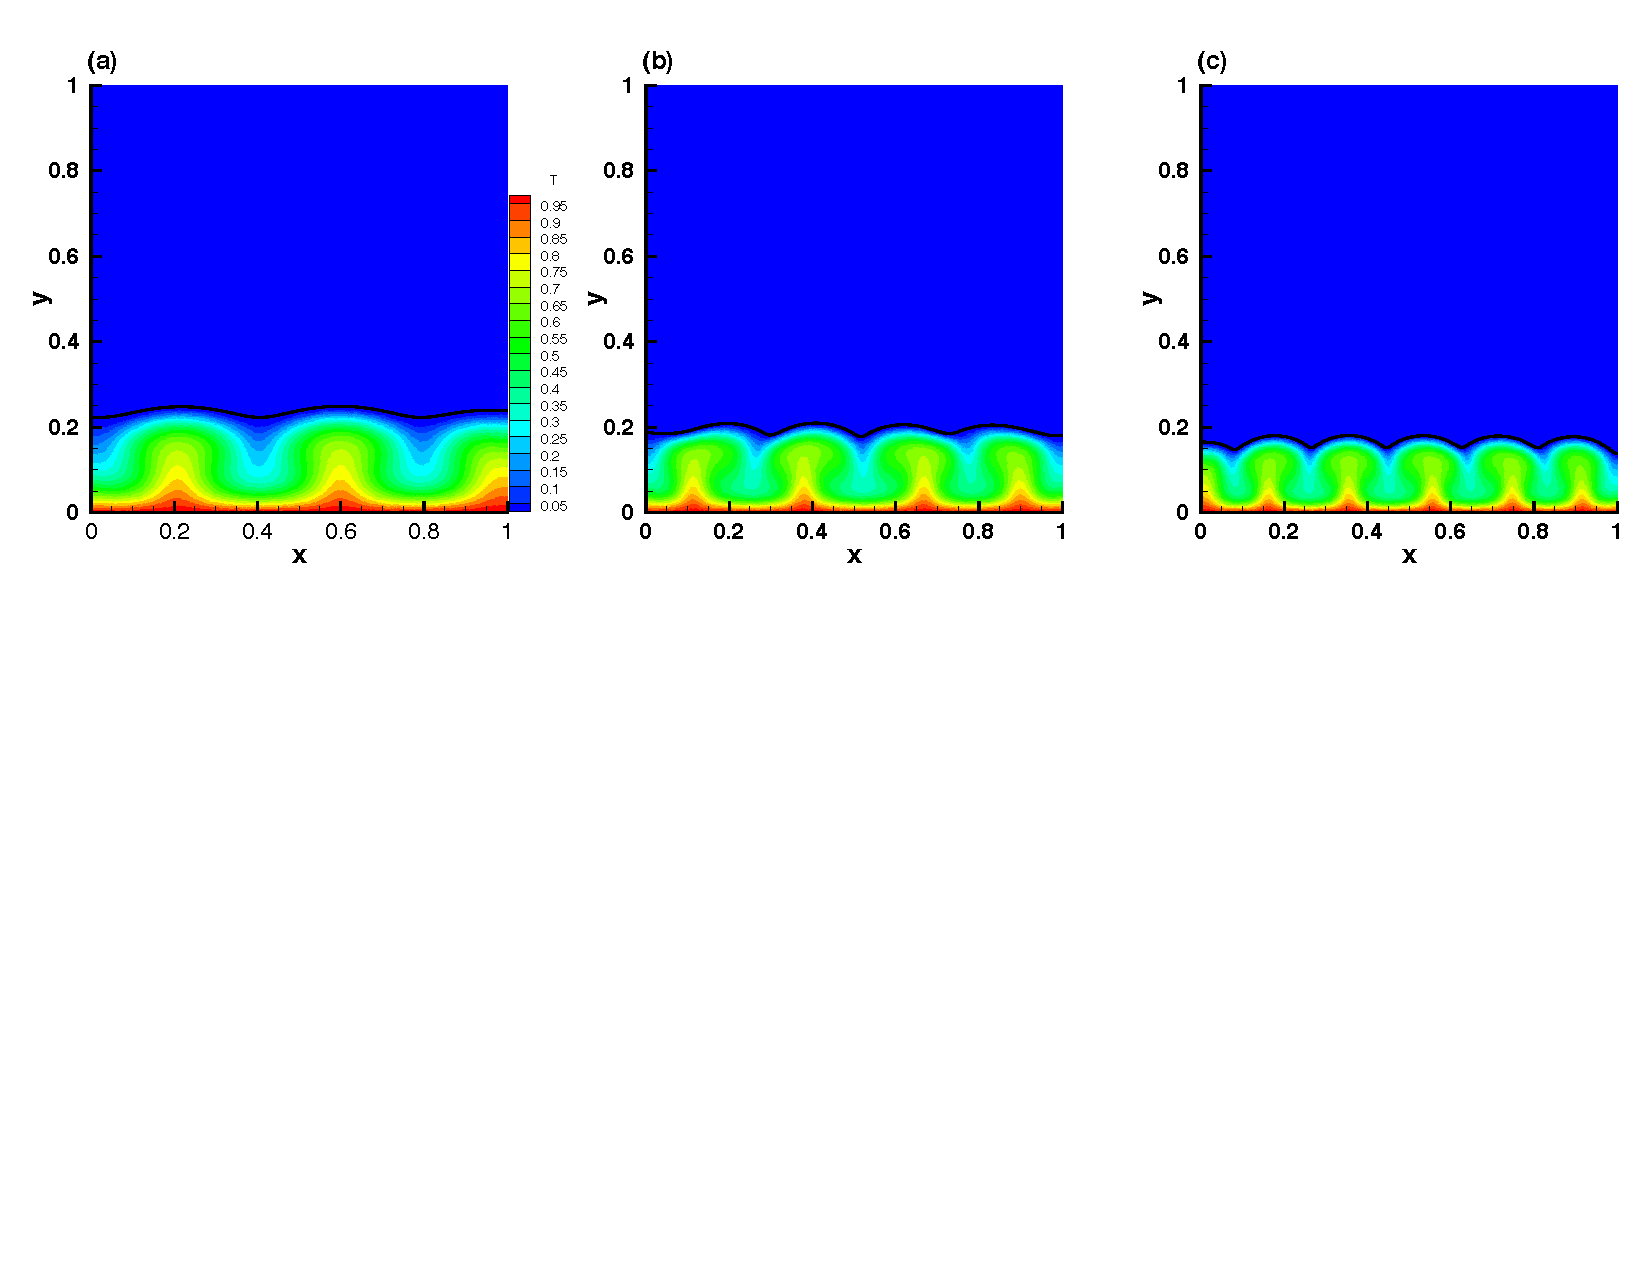
\includegraphics[width=\textwidth]{\figpath/Fig_cap_melting_basal/T_MELT_BASAL_heating}
	\end{center}
	\caption{Melting of PCM heated from below: Temperature field and solid-liquid interface for different size of the domain. (a) $\Ray = 3.27 \cdot 10^5$, (b)  $\Ray = 1.62 \cdot 10^6$, (c) $\Ray = 3.27 \cdot 10^6$.}
	\label{fig:melt-below}
\end{figure}



